\section{Sampling}

Under certain conditions,
a CT signal can be completely
represented by and recovered from
a set of sampled values. This fact
shocked me when I first heard it.
In general, if you consider
$n$ points, you would expect that
infinitely many possible CT signals
could pass through the given points,
as in Figure \ref{fig:sampling_ambiguity}.
\begin{figure}[htbp]
    \centering
    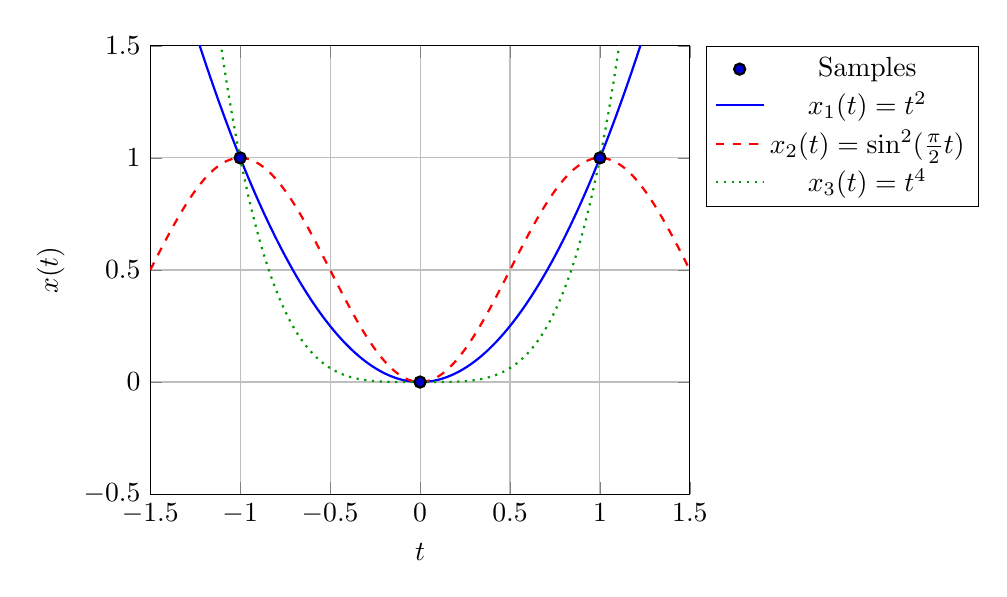
\begin{tikzpicture}
        \begin{axis}[
                xlabel={$t$},
                ylabel={$x(t)$},
                xmin=-1.5, xmax=1.5,
                ymin=-0.5, ymax=1.5,
                legend pos=outer north east,
                grid=major,
                samples=100, % Increase samples for smoother curves
                smooth,      % Use smooth plotting
            ]

            % Plot the sample points
            \addplot+[only marks, mark=*, mark size=2pt, thick, black]
            coordinates {(-1,1) (0,0) (1,1)};
            \addlegendentry{Samples}

            % Plot the first function: x^2
            \addplot[domain=-1.5:1.5, blue, thick] {x^2};
            \addlegendentry{$x_1(t) = t^2$}

            % Plot the second function: sin^2(pi/2 * t)
            % Need deg() because pgfplots trig functions expect degrees by default
            \addplot[domain=-1.5:1.5, red, dashed, thick] {sin(deg(pi/2*x))^2};
            \addlegendentry{$x_2(t) = \sin^2(\frac{\pi}{2}t)$}

            % Plot the third function: t^4
            \addplot[domain=-1.5:1.5, green!60!black, dotted, thick] {x^4};
            \addlegendentry{$x_3(t) = t^4$}

        \end{axis}
    \end{tikzpicture}
    \caption{Sampling Ambiguity}
    \label{fig:sampling_ambiguity}
\end{figure}
The conditions under which a set of
samples uniquely determine a CT signal
is if its Fourier transform is zero
outside a finite band of frequencies,
and if the samples are taken sufficiently
close together in relation to the highest
frequency present in the signal. The result
is known as the \emph{sampling theorem}, and
it is both surprising and extremely useful.

\subsection{Sampling Theorem}
Let $x(t)$ be a band-limited signal with
$X(j\omega) = 0$ for $|\omega| > \omega_M$.
Then $x(t)$ is uniquely determined by its samples
$x(nT)$, $n = 0, \pm 1, \pm 2, \dots$ if
\begin{equation}
    \omega_s > 2 \omega_M,
\end{equation}
where
\begin{equation}
    \omega_s = \frac{2\pi}{T}.
\end{equation}
Given these samples, we can reconstruct
$x(t)$ by generating a periodic impulse
train in which succesive impulses have amplitudes that are
successive sample values. This impulse train is
then processed through an ideal lowpass filter
with gain $T$ and cutoff frequency greater than $\omega_M$ and
less than $\omega_s - \omega_M$.
The resulting output signal will exactly equal $x(t)$.